\chapter{System Overview}
\label{ch:system}

\section{Introduction}
This chapter presents a detailed overview of the RWU-RV64I processor system that serves as the target platform for the toolchain developed in this work.  
The design originates from the open repository maintained by Prof.\ Dr.-Ing.\ Andreas Siggelkow at Hochschule Ravensburg-Weingarten~\cite{siggelkow-rwu-rv64i}.  
It implements the base RISC-V 64-bit integer instruction set (RV64I)~\cite{riscv-spec} in a compact, single-cycle, Harvard-architecture processor optimized for educational use and toolchain research.  

The chapter first outlines the top-level architecture and module hierarchy, followed by the memory organization, peripheral mapping, and clock structure.  
Finally, the hardware–software integration and simulation environment are discussed.

\section{Top-Level Architecture}
The RWU-RV64I is organized as a modular SoC-style architecture composed of a 64-bit RISC-V CPU core, instruction and data memories, peripheral interfaces, and a JTAG-based debug unit.  
All components are interconnected via a pair of 64-bit system buses — the \textit{Instruction Bus (I-Bus)} and \textit{Data Bus (D-Bus)} — forming a Harvard architecture that allows simultaneous instruction fetch and data access. The block diagram of the RWU-RV64I processor, shown in Figure~\ref{fig:rwu_blockdiagram}, illustrates the overall architectural organization, highlighting the key components and their interconnections within the processor design.

\begin{figure}[H]
  \centering
  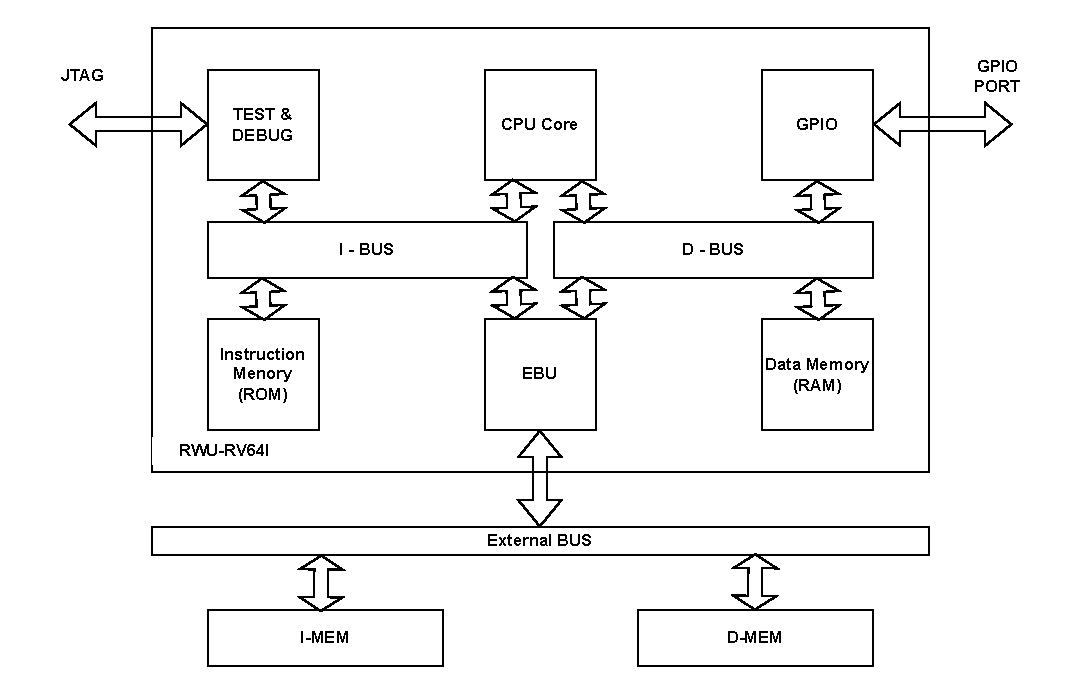
\includegraphics[width=0.9\textwidth]{Thesis_Report/figures/rwu_blockdiagram.pdf}
  \caption{Block-level organization of the RWU-RV64I system.}
  \label{fig:rwu_blockdiagram}
\end{figure}

At the top level, the RWU-RV64I comprises the following modules:

\begin{itemize}
  \item \textbf{CPU Core:} Implements the RV64I instruction set and forms the computational heart of the processor. It includes the register file, ALU, immediate generator, control unit, and program counter logic.
  \item \textbf{Instruction Memory (IMEM):} Stores program instructions and is accessed via the I-Bus.
  \item \textbf{Data Memory (DMEM):} Stores data, variables, and stack content, accessed through the D-Bus.
  \item \textbf{GPIO:} Provides simple 8-bit general-purpose I/O for external interfacing and program verification.
  \item \textbf{External Bus Unit (EBU):} Extends connectivity to external memory or I/O devices beyond the FPGA.
  \item \textbf{Test \& Debug Unit:} Implements JTAG (IEEE 1149.1) for boundary scan and on-chip debugging. The JTAG unit is used as a program loader for the Processor.
\end{itemize}


\section{CPU Core Architecture}
The internal structure of the CPU core is illustrated in Figure~\ref{fig:rwu_core}.  
It contains all fundamental building blocks required for the execution of RV64I instructions.

\begin{figure}[H]
  \centering
  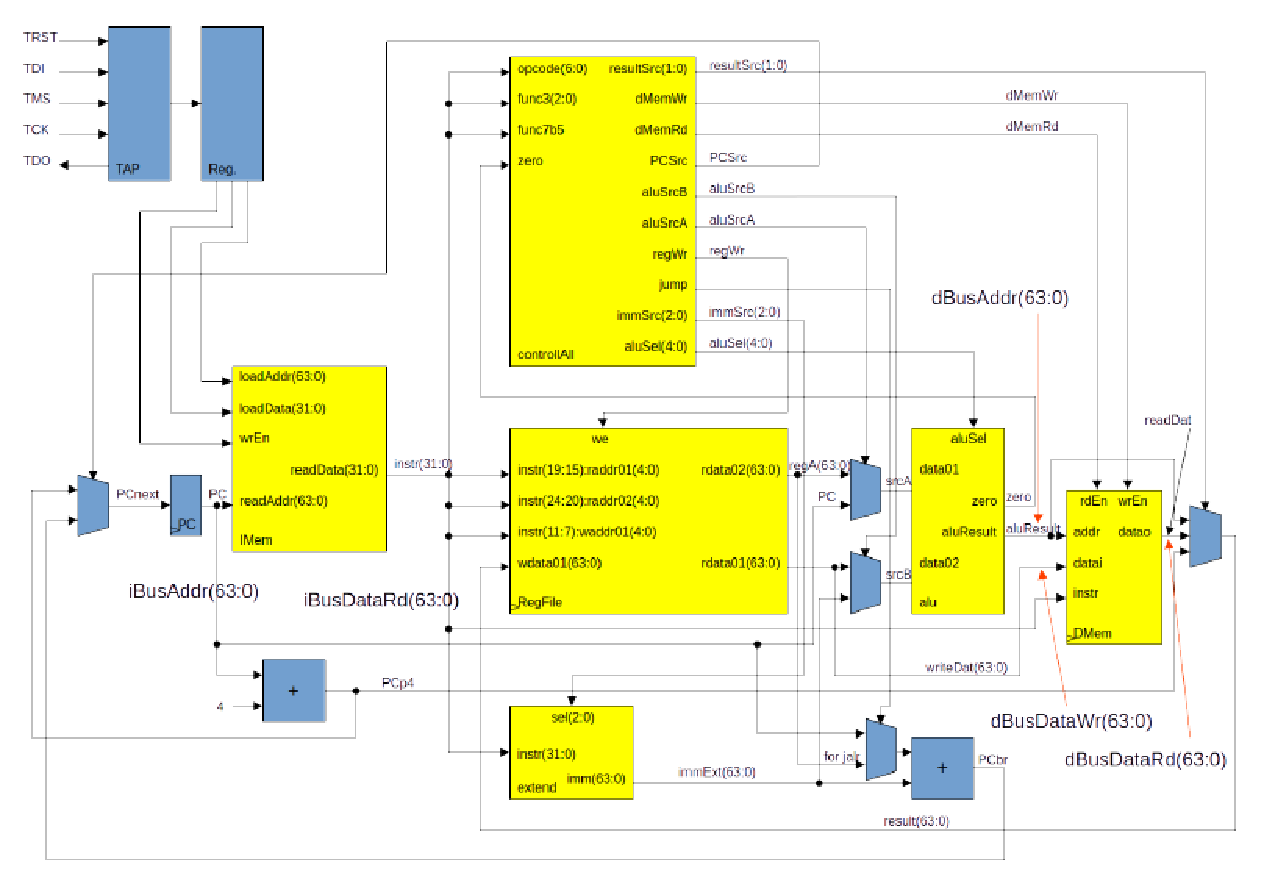
\includegraphics[width=0.95\textwidth]{Thesis_Report/figures/rwu_core.pdf}
  \caption{Datapath and control flow inside the RWU-RV64I CPU core.}
  \label{fig:rwu_core}
\end{figure}

The CPU core executes one instruction per clock cycle — fetch, decode, execute, memory access, and write-back occur sequentially within the same cycle.  
This single-cycle design reduces hardware complexity and ensures deterministic timing behavior, which is particularly useful for toolchain development and low-level software debugging.

\subsection{Datapath Components}
\begin{itemize}
  \item \textbf{Program Counter (PC):} Holds the current instruction address; increments sequentially or updates based on branch/jump logic.
  \item \textbf{Instruction Decode:} Extracts opcode, register fields, and immediate types for control signal generation.
  \item \textbf{Register File:} Contains 32 × 64-bit registers (\texttt{x0–x31}); supports dual read and single write.
  \item \textbf{Immediate Generator:} Extends instruction immediates to 64-bit width for ALU operations.
  \item \textbf{ALU:} Performs integer arithmetic, logical, and shift operations. Results are fed to the memory interface or write-back path.
  \item \textbf{Control Unit:} Generates control signals (\texttt{aluSrcA}, \texttt{aluSrcB}, \texttt{regWr}, \texttt{dMemWr}, \texttt{dMemRd}, etc.) to coordinate datapath elements.
  \item \textbf{JTAG TAP Controller:} Allows programmer to load the code to the instruction memory of the processor via \texttt{TCK}, \texttt{TDI}, \texttt{TDO}, \texttt{TMS}, and \texttt{TRST}.
\end{itemize}

\subsection{Control Flow}
At every clock edge, the instruction is fetched from IMEM, decoded, and executed combinationally by the ALU.  
If the instruction involves memory access, the calculated address is forwarded to the data bus.  
After operation completion, the result is written back to the register file in the same clock cycle.

\section{Memory Organization}
\label{sec:memorg}

The RWU-RV64I adopts a strict Harvard architecture, using physically separate instruction and data memories synthesized within the FPGA fabric~\cite{harvard_architecture}.  
This separation enables parallel instruction fetch and data access during each clock cycle, allowing the processor to achieve deterministic single-cycle execution.

Both memory units are mapped to independent buses:
the \textbf{Instruction Bus (I-Bus)} connects the CPU core to the instruction memory,
while the \textbf{Data Bus (D-Bus)} links the core to the data memory and peripherals.
Each bus is 64 bits wide and follows a simple handshake protocol for read and write transactions.

\subsection{Instruction Memory (IMEM)}
The instruction memory stores up to 8192 words of 32 bits (total capacity = 32 KiB).  
It is addressed by the program counter and provides the next instruction combinationally within the same clock cycle.  
During simulation or FPGA synthesis, IMEM is initialized by reading a hexadecimal file using
\texttt{\$readmemh("riscvtest.mem")}, which is generated automatically by the GNU toolchain.  
Since the architecture is single-cycle, instruction fetches are non-pipelined and incur zero wait states.

\begin{itemize}
  \item \textbf{Word size:} 32 bits  
  \item \textbf{Address width:} 15 bits (lower 2 bits are ignored)  
  \item \textbf{Capacity:} 32 KiB  
  \item \textbf{Access type:} Combinational (read-only)  
  \item \textbf{Initialization:} \texttt{\$readmemh()} from toolchain output
\end{itemize}

\subsection{Data Memory (DMEM)}
The data memory forms the main storage element for program variables and intermediate computational data within the RWU-RV64I processor.  
It consists of 1024 entries, each 64 bits wide, providing a total capacity of 8~KiB. The memory supports fully synchronous read and write operations, ensuring predictable timing behavior during instruction execution.

A byte-select mechanism enables subword data accesses for operations such as \texttt{LB}, \texttt{LH}, \texttt{LW}, and \texttt{LD}, allowing precise manipulation of individual bytes or words within a 64-bit word.  
This design ensures proper alignment and compliance with the RISC-V load/store architecture.

\begin{itemize}
  \item \textbf{Word size:} 64~bits  
  \item \textbf{Address width:} 13~bits  
  \item \textbf{Capacity:} 8~KiB  
  \item \textbf{Access type:} Synchronous read/write  
  \item \textbf{Byte enables:} 8-bit granularity for subword operations
\end{itemize}

The data memory is connected to the system’s address decoder, which identifies whether an access targets internal RAM or a peripheral-mapped region such as GPIO or clock control.  
This modular structure allows easy extension of the memory subsystem to include additional peripherals or external memory interfaces within the same unified address space.


\subsection{Memory Map Overview}
The overall address space seen by the RWU-RV64I processor is summarized in Table~\ref{tab:memmap}.
Each region is selected by the address decoder, which generates the corresponding chip-select signals (\texttt{cs[3:0]}).

\begin{table}[H]
\centering
\caption{Memory map and peripheral address ranges.}
\label{tab:memmap}
\begin{tabular}{lll}
\toprule
\textbf{Address Range} & \textbf{Mapped Device} & \textbf{Chip Select}\\
\midrule
\texttt{0x0000\_0000–0x0000\_FFFF} & Data memory (DMEM) & CS[0]\\
\texttt{0x0001\_0000–0x0001\_000F} & GPIO peripheral & CS[1]\\
\texttt{0x0001\_0010–0x0001\_001F} & Reserved (QSPI) & CS[2]\\
\texttt{0x0001\_0020–0x0001\_002F} & Clock Generation Unit (CGU) & CS[3]\\
\bottomrule
\end{tabular}
\end{table}

Figure~\ref{fig:rwu_memorymap} graphically illustrates this address layout.  
The memory map is linear, beginning with internal data memory at the base address and extending upward to peripheral regions.  
Although the instruction memory resides in a separate Harvard domain, it is shown conceptually for completeness.

\begin{figure}[H]
  \centering
  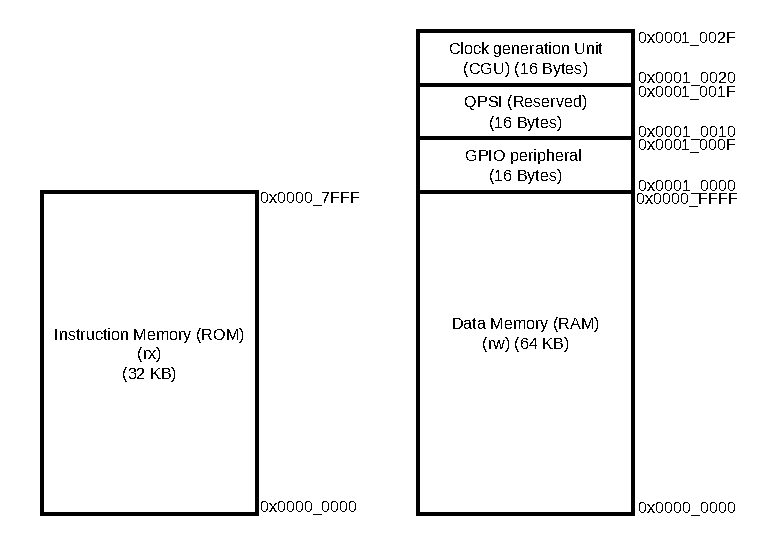
\includegraphics[width=0.85\textwidth]{Thesis_Report/figures/rwu_memorymap.pdf}
  \caption{Memory and peripheral map of the RWU-RV64I.}
  \label{fig:rwu_memorymap}
\end{figure}

The linker script used by the GNU toolchain mirrors this map exactly.  
The \texttt{.text} section occupies IMEM starting from address 0, while data sections (\texttt{.data}, \texttt{.bss}) are placed in DMEM after a 256-byte reserved region used for runtime bookkeeping.  
This tight correspondence ensures that compiled C programs access the correct physical addresses during both simulation and FPGA execution.

\section{Peripherals}
\subsection{General-Purpose I/O (GPIO)}
The GPIO peripheral provides an 8-bit register accessible at address \texttt{0x0001\_0004}.  
Software can write to this register to toggle LEDs or output status codes.  
It is primarily used for simple program verification during simulation and FPGA testing.

\subsection{Clock Generation Unit (CGU)}
The CGU divides the incoming 125 MHz clock from the Zybo board into several programmable frequencies.  
Configuration registers are memory-mapped at \texttt{0x0001 0020 – 0x0001 002F}.  
Typical settings are shown in Table~\ref{tab:cgu}.

\begin{table}[H]
\centering
\caption{Example CGU division settings.}
\label{tab:cgu}
\begin{tabular}{lll}
\toprule
\textbf{Divider} & \textbf{Output Frequency} & \textbf{Typical Use}\\
\midrule
2 & 62.5 MHz & CPU core\\
25 & 5 MHz & QSPI or slow I/O\\
200 & 625 kHz & Low-speed tests\\
400 & 312 kHz & Minimal power simulation\\
\bottomrule
\end{tabular}
\end{table}

\section{Target Hardware Platform}
All FPGA-based verification was carried out on the Digilent Zybo Z7 (Zynq-7010) board~\cite{zybo-datasheet}.  
The RWU-RV64I subsystem is implemented entirely in the programmable logic, while the ARM Cortex-A9 PS remains idle.  
The GPIO outputs are connected to on-board LEDs and JD port, and the 125 MHz oscillator provides the master clock.


\section{Simulation and Verification Environment}
Functional verification is performed using Vivado’s \texttt{xsim} simulator with the help of testbench's.  
The toolchain-generated memory image (\texttt{riscvtest.mem}) is loaded into IMEM before simulation starts.  
Reset is deasserted after initialization, and the processor executes instructions cycle-by-cycle.  
Correct functionality is verified by monitoring GPIO outputs that follow a predefined sequence.


Observed signals include the instruction and data bus transactions, ALU results, and peripheral activity.  
Waveforms are analyzed using Vivado’s built-in viewer or GTKWave for detailed timing inspection.

\section{Summary}
The RWU-RV64I is a 64-bit, single-cycle RISC-V processor tailored for educational and research use.  
Its modular RTL design—consisting of the CPU core, separate instruction and data memories, GPIO, and clock generation—enables full system visibility and rapid iteration during toolchain testing.  
The deterministic timing and simple bus structure make it ideal for compiler validation, C-runtime debugging, and bare-metal firmware development.  
This system forms the foundation for the software toolchain and evaluation work described in the subsequent chapters.
